\section{ICN-IoT Middleware Design}
In this section, we present the overall ICN-IoT middleware design. It consists of three system components, as shown in Figure~\ref{fig:phy}-- Embedded Device, Aggregator, Local Service Gateway, and IoT server, which offer five principle middleware functionalities, including device discovery, device naming service, IoT service discovery and Pub/Sub management.
%to develop IoT middleware over ICN network.
In contrast to centralized or overlay-based implementation in the legacy IP-based IoT platform, our ICN-IoT architecture pushes these middelware functionalities down to the distributed components to enable self-configuring subsystem to provide not only local services but can also scale to large IoT service enablement.
%In legacy IP-based IoT platform, these functionalities are almost implemented on a centralized server, or over-lay application. In our ICN-IoT middleware architecture, they are pushed down to distributed components which can form a self-configuring subsystem to provide local service as well as a complete system that enables global communication.
\begin{figure}
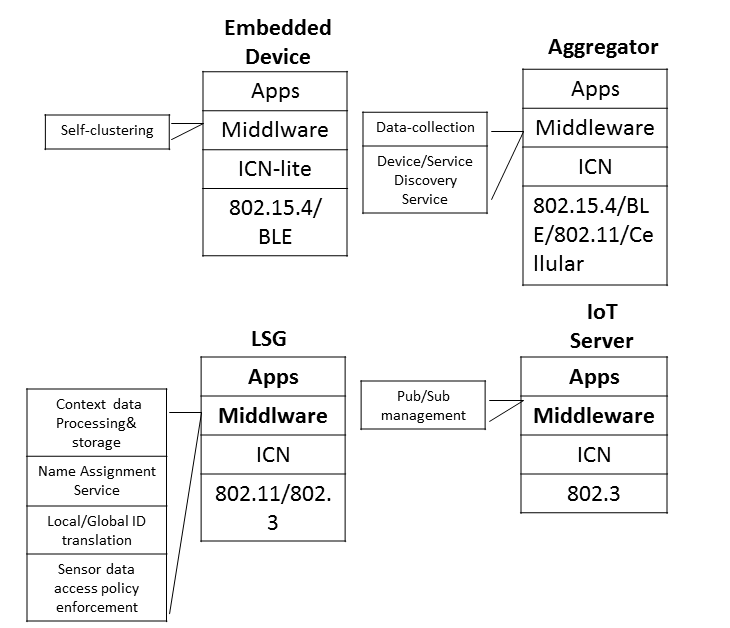
\includegraphics[width=\columnwidth]{figure/physical_comp.png}
\caption{\label{fig:phy}Physical components of ICN-IoT middleware}
\end{figure}

\subsection{System Architecture}\label{sec:physical}

The proposed architecture has the following three main system components:
\begin{itemize}
%\vspace{-2pt}
\item{\em Embedded Device}, which enables seamless ICN protocol in resource-constraint network. A ICN embedded device supports at least one of following communication mode: transmitting and routing over the data to the Aggregator, or responding the request based on name or ID. 
\item{\em Aggregator}, which interconnects various IoT services and content in a local network. An Aggregator usually plays two roles: one is to act as the gateway to bridge the communication between resource-constrained wireless sensors and the rest of the nodes in the local network,  and the other one is to integrate sensing/actuating services in the local network.

%for resource-constraint wireless sensors, or it can be a device that integrates sensing/actuating service.

%\vspace{-2pt}
\item{\em Local Service Gateway (LSG)}, which connects the local IoT system to the rest of the global IoT system, and handles local name assignment and enforces  data access policies for local IoT devices. In addition, it can run context processing services to publish only the contextual information (instead of raw data) to the IoT server.
%It connects local IoT system to the outside world. It handles local name assignment and sensor data access policy enforcement. Furthermore, context data processing service can be implemented within this entity to publish only the information abstraction to IoT server.

%\vspace{-2pt}
\item{\em IoT Server}, which is a centralized server that maintains subscription memberships and provides the lookup service for subscribers. Unlike legacy IoT servers that are involved in the data path from publishers to subscribers -- raising the concern of its interfaces being a bottleneck -- the IoT server in our architecture is only involved in the control path where publishers and subscribers exchange their names and certificates.

%Legacy IoT server also involves in the data path from publisher to subscriber, where the bandwidth of its interfaces could be a bottleneck. In contrast, IoT server in our architecture only involves in control path in which publishers and subscribers exchange their names and certificates.
\end{itemize}

In the following subsections, we will discuss the functionality for each system component (shown as Figure~\ref{fig:phy}) and present detailed protocol design considering NDN and MF.

\subsection{Device Discovery}
The objective of device discovery is to establish connection for nodes in proximity. Device discovery is a key component of any IoT system, and can be considerably simplified by the ICN network. In today's IoT systems, the IP overlay implementation requires a name translation service to maintain the mapping from network addresses to physical attributes, which often involves manual configuration. In ICN-IoT, however, device discovery does not involve any manual configuration or name translation because ICN directly uses names to discover new devices. In what follows, we explain the ICN-IoT device discovery  in detail, including both devices that are able to run  full-stack protocols (referred to as \emph{resource-rich sensors}) and devices that are unable to do so (referred to as \emph{resource-constrained sensors}).

\vspace{1mm}\noindent{\bf Resource-rich sensors}: Many a resource-rich sensor comes with a manufacture secure ID and model name, which needs to be exposed to both the aggregator and LSG to facilitate device discovery. This aim can be achieved by different means with respect to NDN and MF.  In NDN, this process is initiated by the configuration service running on LSG, which periodically broadcasts discovery Interests (using the name $/iot/model$). The new sensor replies to the discovery interest with its information, and the configuration service then registers the sensor and generates a local ICN name for the sensor. In MF, we can set $group$-$GUID$ as the destination address, and the configuration service issues a request via multicasting. When receiving such request, the new device replies with the manufacture secure ID, and the configuration service registers the device and  generates a local ICN name for it.


\vspace{1mm}\noindent{\bf Resource-constrained sensors}: Many resource-constrained sensors connect to the Internet using the IEEE 802.15.4 technology via a border router~\cite{hui2008ip}. These sensors voluntarily discover each other in proximity and establish forwarding paths to the border router by self-organizing into a mesh network. Similarly, for our ICN-IoT middleware,  Aggregator acts as a border router, and neighbor discovery among sensors can be achieved differently with respect to NDN and MF as follows. In NDN, when a new sensor arrives, it broadcasts a neighbor discovery message to connect with neighbors. After establishing connectivity with neighboring sensors, it broadcasts an Interest named $/ndn/aggregatorservice$ to discover the Aggregator. In MF, neighbor discovery is naturally supported, and the new sensor simply needs to send a discovery request to a well-known broadcast GUID to discover the Aggregator. %On receiving, the destination Aggregator receives the request and registers the new device if there is matched service name.
The above process is shown as Figure~\ref{fig:device_dis}
%\footnote{This figure is for either NDN or MF, or both?  The similar question for Figure 6}.
\begin{figure}
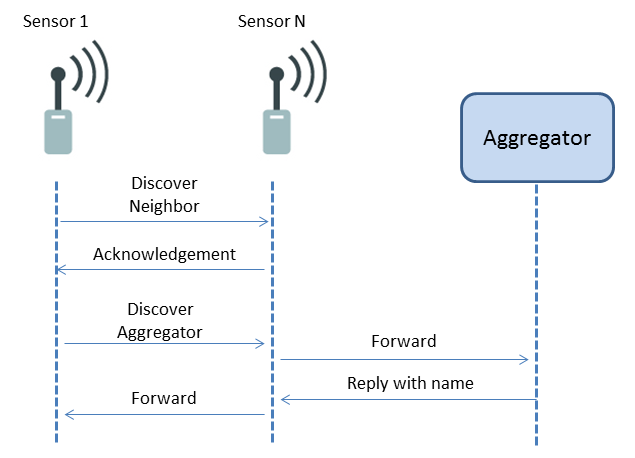
\includegraphics[width=\columnwidth]{figure/device_discovery.png}
\caption{\label{fig:device_dis}Device discovery for resource-constrained sensor}
\end{figure}



\subsection{IoT Service Discovery}

IoT services can be generally categorized into two classes: sensing and actuating. In today's IP based IoT platforms, sensors are connected via a server, which requires considerable development effort such as maintaining a local name to IP mapping. In ICN-IoT, IoT service discovery and configuration becomes much simpler. Specifically, we consider two service discovery modes: $peer$-$to$-$peer$ and $master$-$slave$.


\vspace{1mm}\noindent{\bf Peer-to-peer Service Discovery}: In this mode, we consider the scenario in which an aggregator (referred to as the source aggregator) tries to discover an IoT service provided by another peer aggregator (referred to as destination aggregator). In NDN, the source aggregator broadcasts an interest using the well-known name $/area/servicename/certificate$, which will eventually reach the destination aggregator. NDN's Interest/Data mechanisms allows only one response for each Interest send while discovery requires to learn multiple entities, hence efficient discovery is realized by using exclusion via Selector in the protocol or as an overlay protocol~\cite{ravindran2013information}. In MF, this is handled by multicast (discussed in Section~\ref{sec:intro_mf}) instead of flooding the entire local network. All sensors that provide relevant services can join the multicast group identified by a $Group$-$GUID$. After establishing the multicast group, the source aggregator sends a request containing the service name and certificate to the multicast group.The destination aggregator that hosts the service checks the certificate and registers the source Aggregator if there is a matched service. It replies with an acknowledgement containing its certificate to the source aggregator. The message flow is shown as Figure~\ref{fig:ser_dis}.
\begin{figure}
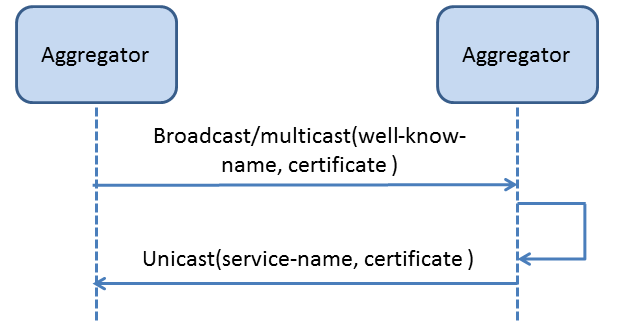
\includegraphics[width=\columnwidth]{figure/service_discovery.png}
\caption{\label{fig:ser_dis}Peer-to-peer service discovery}
\end{figure}
For an example of NDN smart home, a thermostat expresses a request to discover a air conditioning (AC) service using well-known name $/home/ac/certificate$ via broadcast channel. In MF case, a multicast group GUID $1234$ can be assigned to all home appliance IoT service. The thermostat sends request containing the service name and certificate to $1234$. In both cases, the AC hosting this services replies with acknowledgement if all conditions match.

\vspace{1mm}\noindent{\bf Master-slave Service Discovery}: In some IoT applications, there are more than one sensing service or actuating service connecting to one control service. A source aggregator hosting control service expresses a request with service name and its certificate to discover a service from all  available aggregators. The destination aggregators verify the certificate. If valid, the destination aggregators register the source aggregator and  answer with acknowledgement containing their certificates if there is a matched service.

In the AC control NDN example, the number of AC service provider increases to three, which can be named as $/office/ac/1$, $/office/ac/2$ and $/office/ac/3$ . The thermostat expresses a partial name $/office/ac/certificate$ via a broadcast channel periodically. In the MF case, a multicast group GUID $1234$ can be assigned to identify AC service. The thermostat sends request with service name and certificate to $1234$. The destination ACs reply with their certificate if the request meets all criteria.
\subsection{Data Aggregation and Context Data Processing}
Compare to traditional communication networks, IoT networks introduce redundant low-rate data, and many-to-one data flow. Thus, data aggregation is necessary in this setting for energy and bandwidth efficient message flow. Moreover, context information such as time and device location, can be used towards processing logic. Note that context processing is application-centric, hence specific data processing logic depends on the specific IoT application. Aggregator provides first level redundant data filtering from the attached sensors, and adapts the data to heterogeneous application requirement. At the next level component, LSG supports domain-based context processing based on location and device type.

\subsection{Device/App Naming service}  
Naming service is an important function especially for ICN-IoT due to its naming feature. Basically, naming service is responsible for assigning ICN names to the devices and services when the devices are connected to the network or the Apps are deployed in the network environment, and providing name lookup/resolution if necessary. In addition, it is essentailly important to secure the naming service because unprotected (or insecure) naming service might open the door to potential attacks, such as sybil (or spoofing) attack \cite{sybil} with forged names.
 
In what follows, let us consider the approach of building secure naming service in ICN-IoT. Suppose that the device (i.e., sensor) can be either programmable so that before deployment the owner can preload some identity information (such as secure ID, a pair of public/private key and a certificate) , or has some manufacture ID and a pair of public/private key (which is certified by the manufacturer). That is, the device is associated with some information including device identity, public/private keys ($PK_{device}, SK_{device}$) and a certificate either from the owner or the manufacturer that certifies the device identity and public/private keys. For the ICN-IoT middleware on top of NDN, when discovering a device, the aggregator will first verify the device identity (e.g., the device can generate a signature with the private key $SK_{device}$ and present the signature and the certificate to the aggregator so that the aggregator can verify it), and then assign an ICN name to the device as follows: the aggregator will issue a request to LSG together with its device identity and $PK_{device}$, so that LSG can assign an ICN name and generate a certificate (certifying the binding of ICN name, $PK_{device}$). To this end, the ICN name and the certificate will be sent back to the aggregator and will be stored locally if the device is resource-restricted. Otherwise, the ICN name and the certificate will be passed to the device. We note that through this process, ICN name is tightly binding with the device so that sybil attack cannot work. For the MF-IoT, assigning a network name (GUID) for a device is rather straightforward: after verifying the device identity, the Aggregator
inserts the public key $PK_{device}$ and device information to the upper layer component to verify if there is a conflict in the corresponding scope. Specifically, LSG is in charge of local scope and IoT server guarantees the global uniqueness. Finally, the unique public key is used a GUID for the new device. Analogously, assigning ICN names to the Apps can be done in a similar way.
 
In the case where devices are only associated with the secure manufacture ID while without being pre-loaded public/private keys and the certificates, it is critical to assure that devices are authenticated by using other trust model. For example the system can employ the web-of-trust model so that the devices manufactured by the same vendor can authenticated each other. Moreover, in order to comply with the capability of resource-restricted devices, light-weight cryptographic primitive (such as symmetric cryptography) may be used instead of public key cryptography.

%\subsection{Secured Device Naming Service}
%A key step towards realizing a unified IoT platform is the ability to assign names that are unique within the scope and lifetime of each device, data items generated by these devices, or a group of devices towards a common objective. Naming service is usually triggered by device discovery. For NDN architecture, automatic naming scheme is following the hierarchical manor with minimum assumption -- device is always named after its attached point's name, and every physical component in our ICN-IoT middleware should have at least one name. Figure~\ref{} illustrates how a new device can be named using ICN-IoT middleware on top of NDN architecture. A sensor is being discovered by a nearby Aggregator. This Aggregator generate a key pair issues a request to the LSG with its manufacture ID and public key. On receiving of the request, the LSG generates a certificate and an ICN name for the new sensor, then send back to the Aggregator. Last, the Aggregator forward the information to the sensor or store it if the sensor has limited resource. In MF, generating a GUID for a new sensor is rather straightforward: the nearby Aggregator generates a key pair for the sensor, and inserts the public key and device information to the upper layer component to verify if there is a conflict in the corresponding scope. Specifically, LSG is in charge of local scope and IoT server guarantees the global uniqueness.Finally, the unique public key is used a GUID for the new device.


\subsection{Publish/Subscribe Management}
Data Publish/Subscribe (Pub/Sub) is an important function for ICN-IoT, and is responsible for resource sharing and management. In conventional IP network, most of the IoT platforms provide a centralized server to aggregate all IoT service and data. While
%resource is published as service,
this centralized architecture ensures high availability, it scales poorly and has high bandwidth consumption due to high volume of control/data exchange by a central server. Thus, we consider a decentralized pub/sub model in ICN-IoT middleware. Specifically, we will discuss rendezvous mode and a data-control separation mode.

\vspace{1mm}\noindent{\bf Rendezvous Mode}: Rendezvous mode is a classic pub/sub scheme in which data and requests meet at an intermediate node with assistance from a IoT server. While NDN is a Pull-based architecture without supporting the Pub/Sub mode naturally,  COPSS~\cite{chen2011copss} proposes a solution to fix this problem. It integrates a Push-based multicast feature with the pull based NDN architecture at the network layer by introducing Rendezvous Node (RN). RN is a logical entity that resides in NDN forwarder. The publisher first forwards a Content Descriptor (CD) as a snapshot to the RN. RN maintains a subscription table, and receives the Subscription message from subscribers. The data publisher just sends the content using Publish packet by looking up FIB instead of PIT. If the same content prefix is requested by multiple subscribers, RN will deliver one copy  of content downstream, which reduces the bandwidth consumption substantially.

\begin{figure}
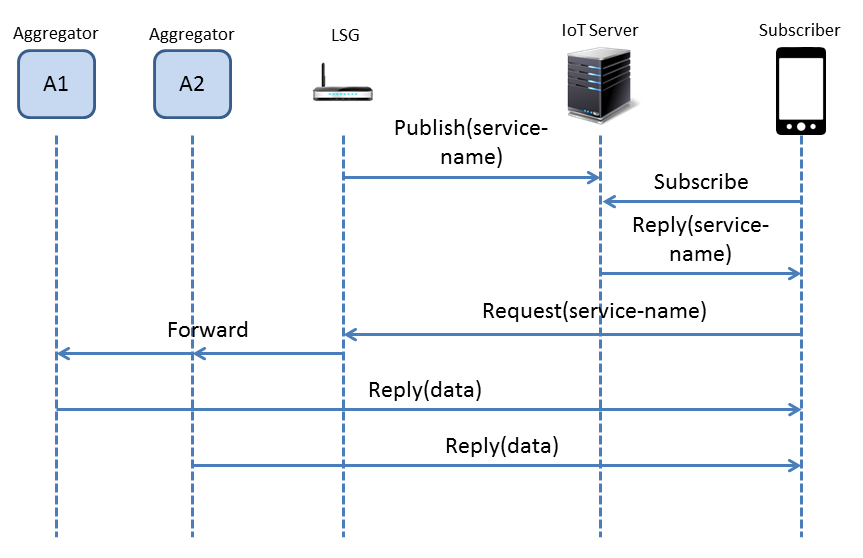
\includegraphics[width=\columnwidth]{figure/pub_sub.png}
\caption{\label{fig:pubsub}Publish/subscriber management message flow}
\end{figure}
\vspace{1mm}\noindent{\bf Data-control separation Mode}: Compared with the Rendezvous mode in which data plane and control plane both reside on the same ICN network layer, we consider an architecture where the control message is handled by the centralized server while data is handled by ICN network layer.  Following the naming process mentioned above, the LSG has the ICN name for the local resource which is available for publishing on IoT server.  IoT server maintains the subscription membership, and receives subscription requests from subscribers. Since the subscribers has non knowlege about the number of resource providers and their identities  in a dynamic scenario,  IoT server has to take responsibility of grouping and assigning group name for the resource. The generic message flow for publish/subscribe function is shown in Figure~\ref{fig:pubsub}, and we will illustrate the detail for NDN and MF.
In NDN, the grouping resource is intuitive: all resources have the same schematic prefix will be grouped together, and the prefix can be used to identify the service. The traditional NDN supports using a common partial name to retrieve multiple resources via Selector, but M. Amadeo et al. ~\cite{amadeo2014multi} provides a more efficient solution to improve this mechanism by introducing long-life multi-source Interest in PIT. MF takes advantage of  $Group$-$GUID$ to identify a service provided by multiple resources. This $Group$-$GUID$ will be distributed to the subscriber as well as the publisher. In an example of NDN,  it uses the common prefix$/home/monitoring/$ to identify a group of resource that provides multiple monitoring services such as $/home/monitoring/temperature$ and $/home/monitoring/light$. The subscriber retrieves the prefix from the IoT server, and sends Interest toward the resource. In a MF example, $GUID$-$x$ identifies the ``home monitoring'' service that combines with ``light status'' and ``temperature''. The resource producers, i.e. the host of ``temperature'' and the host of ``light status'' are notified that their services belong to $GUID$-$x$, then listen on $GUID$-$x$. The subscriber sends the request containing  $GUID$-$x$ through multicasting which ultimately reaches the producers at last common node. Once receiving the request, the resource producer unicasts the data to the subscriber. In addition, if multiple resource consumers subscribe to the same resource, the idea of $Group$-$GUID$ can be reused here to group the consumers to further save bandwidth using multicast.

